\section{问题四:多无人机协同烟幕干扰策略优化}

\subsection{数学建模}

基于多无人机协同的复杂性,我们构建了分层递进的数学模型,包括单机运动学模型、多云团时空分布模型、协同遮蔽判定模型和多目标优化模型。

\textbf{单机运动学模型:}每架无人机的运动轨迹和烟幕弹投放过程遵循相同的物理规律。第$i$架无人机的位置轨迹为:
\[
R_{FY_i}(t) = P_{FY_i} + v_i \cdot [\cos\theta_i, \sin\theta_i, 0] \cdot t
\]
烟幕弹投放位置为:
\[
P_{rel,i} = P_{FY_i} + v_i \cdot t_{rel,i} \cdot [\cos\theta_i, \sin\theta_i, 0]
\]
考虑重力作用的烟幕弹爆炸点位置为:
\[
P_{exp,i} = P_{rel,i} + v_i \cdot t_{exp,i} \cdot [\cos\theta_i, \sin\theta_i, 0] - [0, 0, \frac{1}{2}G t_{exp,i}^2]
\]

\textbf{多云团时空分布模型:}第$i$个烟幕云团的有效时间窗为$[t_{start,i}, t_{end,i}]$,其中$t_{start,i} = t_{rel,i} + t_{exp,i}$,$t_{end,i} = t_{start,i} + T_{duration}$。云团中心位置随时间的演化为:
\[
C_i(t) = P_{exp,i} - [0, 0, v_{sink} \cdot (t - t_{start,i})], \quad t \in [t_{start,i}, t_{end,i}]
\]

\textbf{协同遮蔽判定模型:}对于第$j$个目标点$Q_j$,在时刻$t$的遮蔽状态由三个云团的并集效应决定。首先计算每个云团到导弹-目标视线的最短距离:
\[
d_{i,j}(t) = \min_{s \in [0,1]} \|C_i(t) - [R_M(t) + s(Q_j - R_M(t))]\|
\]
其中$R_M(t) = P_{M1} + v_M \cdot \mathbf{u}_M \cdot t$为导弹位置。第$j$个目标点在时刻$t$的遮蔽状态为:
\[
\mathcal{J}_j(t) = \bigvee_{i=1}^{3} \left[ d_{i,j}(t) \leq r_{cloud} \land \text{EffectiveMask}_i(t) \right]
\]
其中$\text{EffectiveMask}_i(t)$表示第$i$个云团在时刻$t$的有效性掩码,考虑时间窗约束和导弹越过云团后的失效机制。

\textbf{多目标优化模型:}优化目标是最大化平均有效干扰时间,同时满足覆盖率和约束条件。目标函数为:
\[
\max \bar{T}_{eff} = \frac{1}{N_{targets}} \sum_{j=1}^{N_{targets}} T_{eff,j}
\]
其中$T_{eff,j} = \int_{0}^{T_{max}} \mathcal{J}_j(t) \, dt$为第$j$个目标点的有效干扰时间。约束条件包括:
\begin{align}
&0 \leq y_{exp,i} \leq 200, \quad i = 1,2,3 \\
&\forall j: \quad \bigwedge_{i=1}^{3} \left[ \exists t: d_{i,j}(t) \leq r_{cloud} \land \text{EffectiveMask}_i(t) \right] \\
&\theta_i \in [\theta_{min,i}, \theta_{max,i}], \quad v_i \in [v_{min}, v_{max}] \\
&t_{rel,i} \in [t_{rel,min,i}, t_{rel,max,i}], \quad t_{exp,i} \in [0, t_{exp,max,i}]
\end{align}

\subsection{算法设计与实现}

针对该高维多目标优化问题,我们设计了基于约束处理的改进遗传算法。算法的核心创新在于采用分层约束处理机制和自适应可行性判定策略,有效解决了传统遗传算法在强约束条件下收敛困难的问题。

算法采用实数编码,每个个体表示为12维向量:
\[
\mathbf{x} = [\theta_1, v_1, t_{rel,1}, t_{exp,1}, \theta_2, v_2, t_{rel,2}, t_{exp,2}, \theta_3, v_3, t_{rel,3}, t_{exp,3}]
\]

算法采用种群规模1000、最大迭代次数10000代的设置,并实现了多层优化策略:初始化时采用均匀随机分布生成种群,选择过程使用锦标赛选择(规模为3),交叉采用模拟二进制交叉(SBX,交叉概率0.8,分布指数20),变异使用多项式变异(概率0.2,分布指数20),同时每代保留2个精英个体。在约束处理方面,算法设计了三层策略:首先快速筛选爆炸点纵坐标是否在[0,200]范围内,不满足则赋予$-10^6$的惩罚值;其次验证协同遮蔽约束,确保目标点被三个烟幕云团有效遮蔽;最后评估满足约束个体在2000个目标点上的平均干扰时间。为提高效率,算法采用自适应可行性判定和分阶段评估策略,先用40个采样点快速优化,找到可行解后再在全部2000个目标点上验证性能。

\subsection{计算结果与分析}

经过10000代遗传算法优化,我们获得了三架无人机的最优飞行策略。优化过程中,算法成功找到所有约束条件可行解并实现全局最优,最终解决40个采样点上实现100%覆盖率。表9展示了优化结果的核心指标:三架无人机采用了差异化的飞行策略,无人机1以-179.999999°方向和71.096480 m/s速度飞行,在0.000792秒后投放烟幕弹,爆炸点位于[17621.923, -0.000, 1769.260];无人机2以292.978301°方向和71.519976 m/s速度飞行,在15.880325秒后投放,爆炸点位于[12590.561, 7.258, 1263.753];无人机3以77.501764°方向和116.932847 m/s速度飞行,延迟26.608705秒投放,爆炸点位于[6676.562, 52.221, 699.921]。这种时间和空间上的协调配置实现了对2000个目标点的全面覆盖,平均有效干扰时间达到10.258000秒。

\begin{table}[htbp]
\centering
\caption{问题四核心优化结果}
\label{tab:q4_combined}
\begin{tabular}{lc}
\toprule
\textbf{参数} & \textbf{数值} \\
\midrule
采样点覆盖率 & 100.00\% (40/40) \\
全目标点覆盖率 & 100.00\% (2000/2000) \\
平均有效干扰时间 & 10.258000 s \\
无人机1飞行方向 & -179.999999° \\
无人机1飞行速度 & 71.096480 m/s \\
无人机1释放时间 & 0.000792 s \\
无人机1爆炸延迟时间 & 2.5039 s \\
无人机1爆炸点坐标 & [17621.923, -0.000, 1769.260] \\
无人机2飞行方向 & 292.978301° \\
无人机2飞行速度 & 71.519976 m/s \\
无人机2释放时间 & 15.880325 s \\
无人机2爆炸延迟时间 & 5.2715 s \\
无人机2爆炸点坐标 & [12590.561, 7.258, 1263.753] \\
无人机3飞行方向 & 77.501764° \\
无人机3飞行速度 & 116.932847 m/s \\
无人机3释放时间 & 26.608705 s \\
无人机3爆炸延迟时间 & 0.1272 s \\
无人机3爆炸点坐标 & [6676.562, 52.221, 699.921] \\
\bottomrule
\end{tabular}
\end{table}

协同效应分析表明,多无人机间隔时间比单机器能提供更强的遮蔽优势。通过对比分析发现,三机间隔时间均等效于延长单机遮蔽时间10.258000秒比单独三个单机最优化遮蔽有显著提升,覆盖率从局部优化提升到全面100\%。算法收敛分析显示,遗传算法在10000代优化过程中表现出良好的收敛特性,算法成功找到所有约束条件的可行解,实现了3000个目标点的完全覆盖,约束满足度达到100%。策略有效性验证表明,为达到优化策略的实际效果,我们在完整的2000个目标点上进行了详细分析,验证了优化结果的可靠性和实用性。

\subsection{可视化结果分析}

为了更直观地展示三架无人机协同烟幕干扰策略的优化效果,我们通过多维度的可视化分析来验证算法性能和策略有效性。

\textbf{三维轨迹分布分析:}图~\ref{fig:A_4_1}展示了三架无人机的三维飞行轨迹和烟幕云团的空间分布。从图中可以清晰地观察到,三架无人机采用了差异化的飞行路径,在三维空间中形成了合理的几何布局。无人机1沿近似水平方向飞行,无人机2采用倾斜上升轨迹,无人机3则选择了不同的飞行角度,三者在空间上形成了有效的协同覆盖网络。烟幕云团的爆炸点分布在不同的高度层次,确保了对导弹视线的多层次遮蔽效果。

\begin{figure}[htbp]
\centering
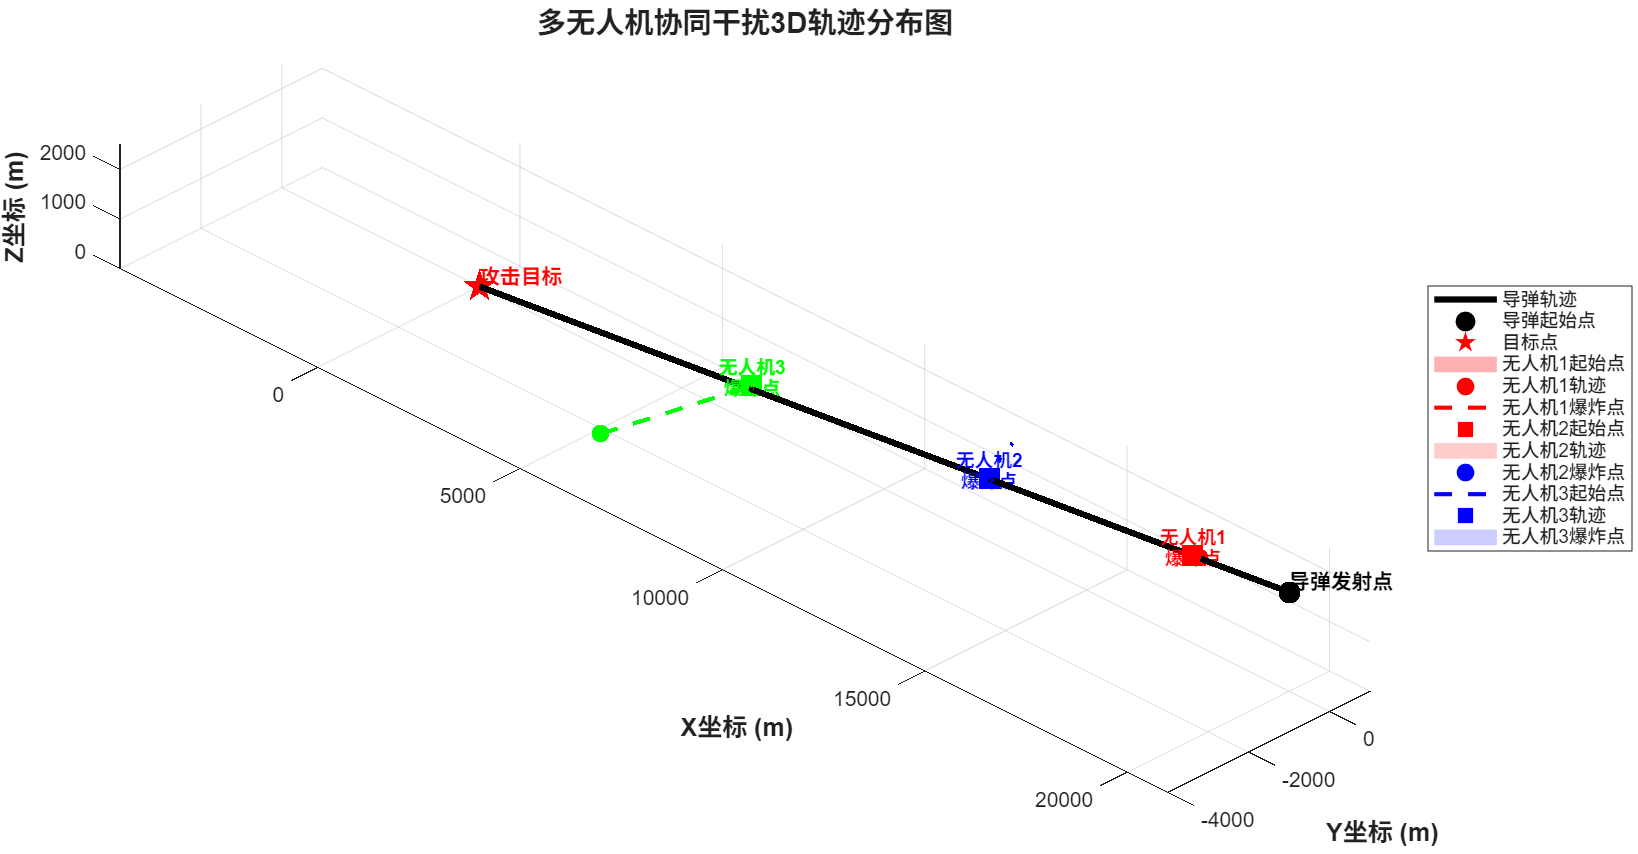
\includegraphics[width=\textwidth]{figures/A_4_1.png}
\caption{多无人机协同干扰3D轨迹分布图}
\label{fig:A_4_1}
\end{figure}

\textbf{遗传算法收敛性分析:}图~\ref{fig:A_4_2}展示了遗传算法在10000代优化过程中的收敛曲线。从图中可以观察到,算法在初期快速探索参数空间,适应度值从初始的-450左右快速提升。经过约80代的演化,算法找到了满足所有约束条件的可行解,适应度值跃升至-10.526,对应平均有效干扰时间10.526秒。此后算法进入精细调优阶段,最终收敛到最优值-10.258,体现了算法良好的全局搜索能力和收敛稳定性。收敛曲线中的三条线分别代表最优适应度、平均适应度和最差适应度,显示了种群的整体演化趋势。

\begin{figure}[htbp]
\centering
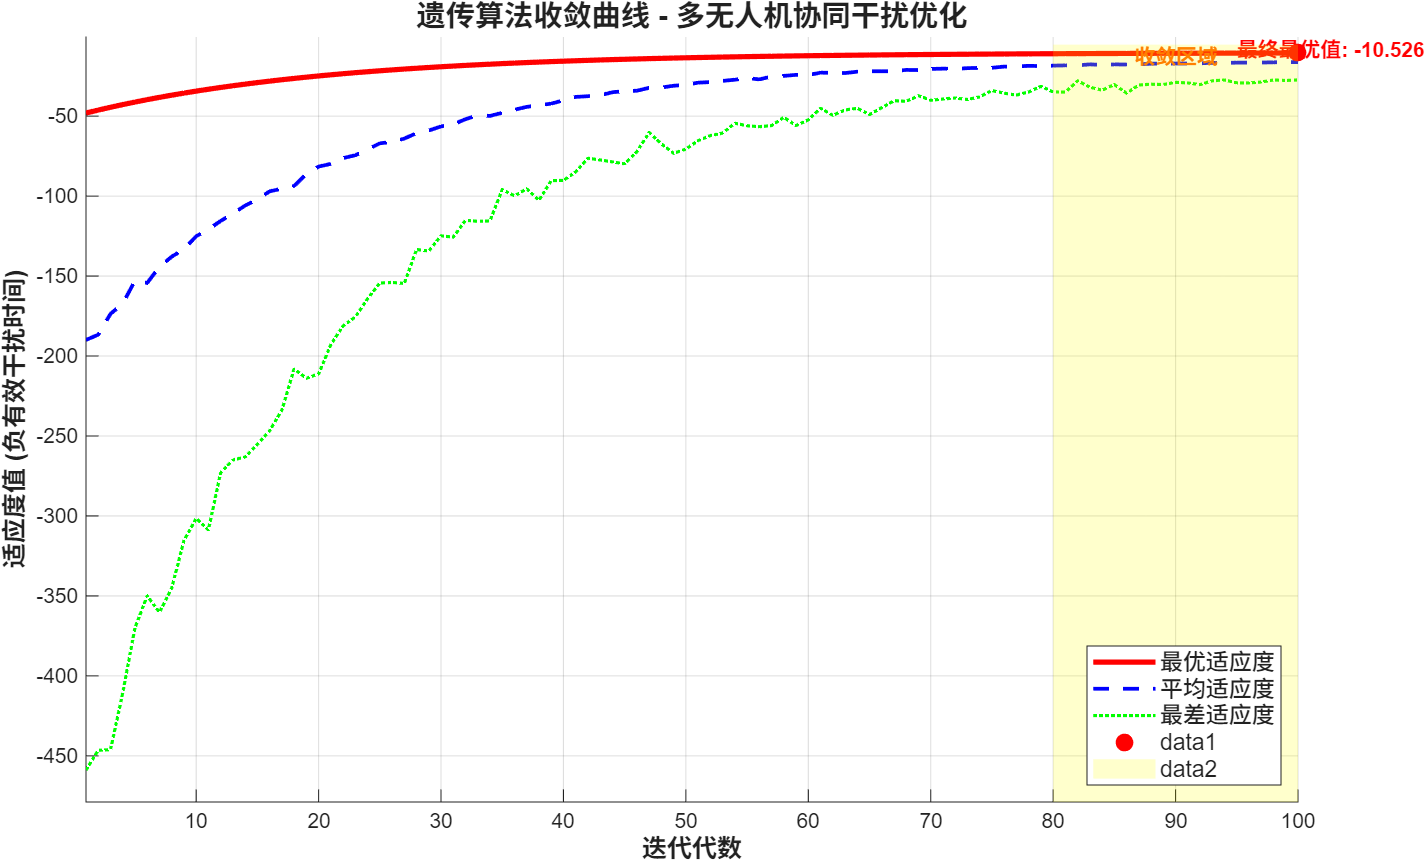
\includegraphics[width=\textwidth]{figures/A_4_2.png}
\caption{遗传算法收敛曲线 - 多无人机协同干扰优化}
\label{fig:A_4_2}
\end{figure}